%
% 3_rechenbeispiel.tex -- Ein einleuchtendes Rechenbeispiel anhand eines einfachen Pendels
%
% (c) 2024 Flurin Brechbühler, OST - Ostschweizer Fachhochschule Rapperswil
%
% !TEX root = ../../buch.tex
% !TEX encoding = UTF-8
%
\section{Rechenbeispiel\label{fem:rechenbsp}}
\kopfrechts{Rechenbeispiel}

Als Rechenbeispiel soll ein einfaches Pendel betrachtet werden. 
Dessen Bewegungsgleichung kann aus der Lagrange-Funktion
\begin{equation}
    L = \frac{1}{2} m l^2 {\theta'}^2 - m g l (1 - \cos \theta),
\end{equation}
mittels der Euler-Lagrange-Differentialgleichung
\begin{equation}
    \theta'' + \frac{g}{l} \sin \theta = 0
\end{equation}
bestimmt werden.

Da wir mit dem bisher behandelten Vorgehen nur lineare Differenzialgleichungen lösen können, wird die Approximation
\begin{equation}
    \sin \theta \approx \theta
\end{equation}
verwendet.
Dies hat jedoch zur Folge, dass die Lösung nur für kleine $\theta$ (ungefähr $\theta < 15 \deg$) gut stimmen wird.

Die Differenzialgleichung, die es zu lösen gilt, ist also
\begin{equation}
    \theta'' + \frac{g}{l} \theta = 0.
\end{equation}
Zudem soll unsere Lösung die Anfangsbedingungen
\begin{equation}
    \theta(0) = 10 \deg
    \quad \text{und} \quad
    \theta'(0) = 0
\end{equation}
erfüllen.
Die Pendelschwingung soll über 4 Sekunden hinweg berechnet werden, der Definitionsbereich $\Omega$ ist also
\begin{equation}
    \Omega = [0\sec, 4\sec].
\end{equation}
Für die Parameter $g$ und $l$ sind die Werte
\begin{equation}
    g = 10
    \quad \text{und} \quad
    l = 1
\end{equation}
gegeben.


\subsection{Bilden der schwachen Form}
Die schwache Form des Problems lautet
\begin{equation}
    \int_\Omega \left( \theta'' + \frac{g}{l} \theta \right) \cdot v \diff t 
    = \int_\Omega \theta'' \cdot v \diff t + \int_\Omega \frac{g}{l} \theta \cdot v \diff t
    = 0
\end{equation}
und kann durch partielles Integrieren des Terms $\int_\Omega \theta'' \cdot v \diff t$ zu einer Differenzialgleichung erster Ordnung gemacht werden:
\begin{equation}
    - \int_\Omega \theta' \cdot v' \diff t + \int_\Omega \frac{g}{l} \theta \cdot v \diff t = -\Phi(\theta, v) = 0
    \label{fem:rechenbsp:schwache_form}
\end{equation}


\subsection{Diskretisieren}
Um den Lösungsweg möglichst übersichtlich zu gestalten, werden die Funktionen $f(t)$ und $\theta(t)$ in $N$ $\Delta t$ lange Stücke unterteilt:
\begin{align}
    f(t) = \sum_{n=0}^{N} f_n \cdot a(t) \quad
    \text{mit} \quad
    f_n = f(n \cdot \Delta t)
\intertext{und}
    \theta(t) = \sum_{n=0}^{N} \theta_n \cdot a(t) \quad
    \text{mit} \quad
    \theta_n = \theta(n \cdot \Delta t).
\end{align}

Zur Interpolation werden lineare Formfunktionen verwendet, da dies die weiteren Rechnungen erleichtert und weil es die Ordnung des zu lösenden Problems erlaubt.
Für $a_n(t)$ ist also mit $t_0 = n \cdot \Delta t$
\begin{equation}
    a_n(t) = \left\{ 
    \def\arraystretch{\formfktStretch}
    \begin{array}{ll}
        1+\frac{t-t_0}{\Delta t} & \text{für} \quad t_0 - \Delta t < t < t_0 \\
        1-\frac{t-t_0}{\Delta t} & \text{für} \quad t_0 \leq t < t_0 + \Delta t \\
        0 & \text{sonst}
    \end{array} \right.
\end{equation}
einzusetzen.


\subsection{Erstellen der Matrix}
Der Vektor $\vec{b}$ ist in diesem Fall besonders einfach zu bestimmen: Da die rechte Seite Null ist, gilt
\begin{equation}
    \vec{b} = \vec{0}.
\end{equation}
Um die Elemente der Matrix $\mathbf{L}$ zu ermitteln, werden die Integrale aus Gleichung \eqref{fem:rechenbsp:schwache_form} verwendet:
\begin{equation}
    l_{ij} = - \int_\Omega a_i'(t) \cdot a_j'(t) \diff t + \int_\Omega \frac{g}{l} a_i(t) \cdot a_j(t) \diff t.
\end{equation}
Im eindimensionalen Fall kann mittels einfacher Bedingungen zwischen den drei Fällen unterschieden werden:
\begin{itemize}
    \item[$i = j$:] Volle Überlappung der Formfunktion: Die Formfunktion wird quadriert und integriert. 
    \item[$|i - j| = 1$:] Die beiden Elemente grenzen aneinander: Es wird über das Produkt der beiden Formfunktionen integriert.
    \item[$|i - j| > 1$:] Die beiden Elemente grenzen nicht aneinander: Die Formfunktionen überlappen nicht, das Integral über das Produkt ist also Null.
\end{itemize}
Bei einem mehrdimensionalen Problem müsste anhand des Graphen ermittelt werden, ob zwei Elemente nebeneinander liegen oder nicht.

\subsubsection{Volles Überlappen ($i = j$)}
Da die Integrale aller Elemente gleich und die Formfunktionen symmetrisch sind, reicht es aus, nur das Integral
\begin{equation}
    \int_{0}^{\Delta t} a_1(t) \cdot a_1(t) \diff t
    = \int_{0}^{\Delta t} \frac{t^2}{(\Delta t)^2} \diff t 
    = \frac{1}{3} \Delta t
\end{equation}
der Formfunktion $ a_1(t) = \frac{t}{\Delta t} $ zu berechnen.
Es resultiert
\begin{equation}
    \int_\Omega a_k(t) \cdot a_k(t) \diff t 
    = 2 \cdot \int_{0}^{\Delta t} a_1(t) \cdot a_1(t) \diff t 
    = \frac{2}{3} \Delta t 
    \quad \text{für} \quad 0 < k < N.
\end{equation}
Dabei werden die Indizes $0$ und $N$ ausgeklammert, da die linke Hälfte der Formfunktion $a_0(t)$ sowie die rechte Hälfte der Formfunktion $a_N(t)$ ausserhalb des Definitionsbereichs liegen und für diese Knotenvariablen folglich
\begin{equation}
    \int_\Omega a_k(t) \cdot a_k(t) \diff t 
    = \int_{0}^{\Delta t} a_1(t) \cdot a_1(t) \diff t 
    = \frac{1}{3} \Delta t 
    \quad \text{für} \quad k = 1 \quad \text{oder} \quad k = N
\end{equation}
gilt.

Für das Integral über die Ableitungen der Formfunktionen resultiert nach dem Gleichen Vorgehen
\begin{equation}
    \int_\Omega a_k'(t) \cdot a_k'(t) \diff t 
    = 2 \cdot \int_{0}^{\Delta t} a_1'(t) \cdot a_1'(t) \diff t
    = 2 \cdot \int_{0}^{\Delta t} \frac{1}{\Delta t} \cdot \frac{1}{\Delta t} \diff t 
    = \frac{2}{\Delta t}
    \quad \text{für} \quad 0 < k < N,
\end{equation}
da $a_1'(t)= \frac{1}{\Delta t}$ wenn $0 \leq t < \Delta t$.
Auch hier werden die Knoten $0$ und $N$ ausgeklammert, denn für diese gilt
\begin{equation}
    \int_\Omega a_k'(t) \cdot a_k'(t) \diff t 
    = \int_{0}^{\Delta t} a_1'(t) \cdot a_1'(t) \diff t
    = \int_{0}^{\Delta t} \frac{1}{\Delta t} \cdot \frac{1}{\Delta t} \diff t 
    = \frac{1}{\Delta t}
    \quad \text{für} \quad k = 1 \quad \text{oder} \quad k = N.
\end{equation}

\subsubsection{Benachbarte Elemente ($|i - j| = 1$)}
Auch hier reicht es aus, eines der Integrale zu berechnen. 
Gewählt wurden ebenfalls aufgrund der einfachen Formfunktionen die Funktionen $a_0(t) = 1 - \frac{t}{\Delta t}$ und $a_1(t) = \frac{t}{\Delta t}$.
Es resultiert
\begin{equation}
    \int_\Omega a_k(t) \cdot a_{k+1}(t) \diff t = \int_{0}^{\Delta t} \left(1 - \frac{t}{\Delta t}\right) \cdot \frac{t}{\Delta t} \diff t = \frac{1}{6} \Delta t.
\end{equation}
Auch hier wird noch das Integral über die Ableitungen 
\begin{equation}
    \int_\Omega a_k'(t) \cdot a_{k+1}'(t) \diff t = \int_{0}^{\Delta t} -\frac{1}{\Delta t} \cdot \frac{1}{\Delta t} \diff t = -\frac{1}{\Delta t},
\end{equation}
benötigt.
Hierbei gilt $a_0'(t)= -\frac{1}{\Delta t} \ \text{und} \ a_1'(t)= \frac{1}{\Delta t} \ \text{wenn} \ 0 \leq t < \Delta t$

\subsubsection{Resultat}
Für die Elemente $l_{ij}$ der Array $\mathbf{L}$ gilt also
\begin{align}
    l_{ij} 
    &= - \int_\Omega a_i'(t) \cdot a_j'(t) \diff t + \frac{g}{l} \int_\Omega a_i(t) \cdot a_j(t) \diff t \notag \\
    &=  \left\{ 
            \def\arraystretch{\formfktStretch}    
            \begin{array}{ll}
                - \frac{1}{\Delta t} + \frac{g}{3l} \Delta t & \text{für} \quad i = j = 0 \\
                - \frac{2}{\Delta t} + \frac{2g}{3l} \Delta t & \text{für} \quad i = j \neq 0 \\
                \frac{1}{\Delta t} + \frac{g}{6l} \Delta t & \text{für} \quad |i - j| = 1 \\
                0 & \text{sonst}
            \end{array} 
        \right. .
\end{align}
Für einen willkürlich gewählten Zeitschritt von $\Delta t = 0.1$ und den in der Aufgabenstellung festgelegten Parametern $g = 10$ und $l = 1$ resultiert das Gleichungssystem
\begin{equation}
    \def\arraystretch{1.5}
    \mathbf{L}\vec{u} + \vec{b} 
    = \begin{pmatrix}
         -9.67  & 10.17  &                &                &        &        \\
         10.17  &-19.33  & 10.17          &                &        &        \\
                & 10.17  &-19.33          & \smash{\ddots} &        &        \\
                &        & \smash{\ddots} & \smash{\ddots} & 10.17  &        \\
                &        &                & 10.17          &-19.33  & 10.17  \\
                &        &                &                & 10.17  & -9.67
    \end{pmatrix}
    \begin{pmatrix}
        u_0 \\ u_1 \\ u_2 \\ u_3 \\ \vdots \\ u_N
    \end{pmatrix}
    +
    \begin{pmatrix}
        0 \\ 0 \\ 0 \\ 0 \\ \vdots \\ 0
    \end{pmatrix}
    = 0.
    \label{fem:rechenbsp:gleichungssystem}
\end{equation}


\subsection{Codieren der Anfangsbedingungen}
Die Anfangsbedingungen
\begin{equation}
    u(0) = 10 \deg \approx 0.175 \radian
    \quad \text{und} \quad
    u'(0) = 0
\end{equation}
werden wie in Abschnitt \ref{fem:1d:anfangsbedingungen} beschrieben in die Matrix eingebracht.
Dazu wird das Gleichungssystem \eqref{fem:rechenbsp:gleichungssystem} zunächst als Gauss-Tableau geschrieben:
\begin{equation}
    \def\arraystretch{1.5}
    \begin{array}{|cccccc|c|}
        \hline
        -9.69  & 10.17  &                &                &        &        & 0              \\
        10.17  &-19.33  & 10.17          &                &        &        & 0              \\
               & 10.17  &-19.33          & \smash{\ddots} &        &        & 0              \\
               &        & \smash{\ddots} & \smash{\ddots} & 10.17  &        & \smash{\ddots} \\
               &        &                & 10.17          &-19.33  & 10.17  & 0              \\
               &        &                &                & 10.17  & -9.67  & 0              \\
        \hline
    \end{array}.
\end{equation}

\subsubsection{$\mathbf{u(0) = 0.175 \radian}$:}
Die einzufügende Gleichung
\begin{equation}
    x_0 = 0.175
\end{equation}
ersetzt also die Zeile $0$:
\begin{equation}
    \def\arraystretch{1.5}
    \begin{array}{|cccccc|c|}
        \hline
        \pivotoperation{0.6cm}{0.2cm}{-0.2cm}{-0.2cm}
         1.00  &        &                &                &        &        & 0.175          \\
        \forwardreduction{0.6cm}{2.9cm}{-0.1cm}{-2.7cm}
        10.17  &-19.33  & 10.17          &                &        &        & 0              \\
               & 10.17  &-19.33          & \smash{\ddots} &        &        & 0              \\
               &        & \smash{\ddots} & \smash{\ddots} & 10.17  &        & \smash{\vdots} \\
               &        &                & 10.17          &-19.33  & 10.17  & 0              \\
               &        &                &                & 10.17  & -9.67  & 0              \\
        \hline
    \end{array}.
\end{equation}
Anschliessend wird noch die Spalte Null gesetzt, indem das $ 10.17 $-fache der ersten Zeile von der zweiten abgezogen wird.
Es resultiert
\begin{equation}
    \def\arraystretch{1.5}
    \begin{array}{|cccccc|c|}
        \hline
         1.00  &        &                &                &        &        & 0.175          \\ 
               &-19.33  & 10.17          &                &        &        & -1.78          \\
               & 10.17  &-19.33          & \smash{\ddots} &        &        & 0              \\
               &        & \smash{\ddots} & \smash{\ddots} & 10.17  &        & \smash{\vdots} \\
               &        &                & 10.17          &-19.33  & 10.17  & 0              \\
               &        &                &                & 10.17  & -9.67  & 0              \\
        \hline
    \end{array}.
\end{equation}

\subsubsection{$\mathbf{u'(0) = 0 }$:}
Hier wird die erwähnte Annäherung zum Codieren der Anfangsbedingung bezüglich der Ableitung angewandt.
Es wird also nicht direkt $u'(0) = 0 $, sondern $u(\Delta t) = u(0) = 0.175 \radian$ codiert.
Es gilt also, zusätzlich die Gleichung
\begin{equation}
    x_1 = 0.175
\end{equation}
in das Tableau einzufügen.
Nach dem gleichen Vorgehen wie bei der vorherigen Randbedingung resultiert
\begin{equation}
    \def\arraystretch{1.5}
    \begin{array}{|ccccccc|c|}
        \hline
         1.00  &        &        &                &                &        &        & 0.175          \\
               &  1.00  &        &                &                &        &        & 0.175          \\
               &        &-19.33  & 10.17          &                &        &        & -1.78          \\
               &        & 10.17  &-19.33          & \smash{\ddots} &        &        & 0              \\
               &        &        & \smash{\ddots} & \smash{\ddots} & 10.17  &        & \smash{\vdots} \\
               &        &        &                & 10.17          &-19.33  & 10.17  & 0              \\
               &        &        &                &                & 10.17  & -9.67  & 0              \\
        \hline
    \end{array},
\end{equation}
was wieder in Vektorschreibweise dargestellt
\begin{equation}
    \def\arraystretch{1.5}
    \mathbf{L}\vec{u} 
    = -\vec{b} 
    = \begin{pmatrix}
         1.00  &        &        &                &                &        &        \\
               &  1.00  &        &                &                &        &        \\
               &        &-19.33  & 10.17          &                &        &        \\
               &        & 10.17  &-19.33          & \smash{\ddots} &        &        \\
               &        &        & \smash{\ddots} & \smash{\ddots} & 10.17  &        \\
               &        &        &                & 10.17          &-19.33  & 10.17  \\
               &        &        &                &                & 10.17  & -9.67  
    \end{pmatrix}
    \begin{pmatrix}
        u_0 \\ u_1 \\ u_2 \\ u_3 \\ u_4 \\ \vdots \\ u_N
    \end{pmatrix}
    =
    \begin{pmatrix}
        0.175 \\ 0.175 \\ -1.78 \\ 0 \\ 0 \\ \vdots \\ 0
    \end{pmatrix}
\end{equation}
ergibt.
Es ist nun auch festzustellen, dass das zu lösende Gleichungssystem für jede Anfangsbedingung um eine Variable kleiner geworden ist, da ja zwei der gesuchten Werte bereits gegeben sind.


\subsection{Invertieren der Matrix}
Mit einem Werkzeug wie Matlab kann die erhaltene Matrix $\mathbf{L}$ invertiert und der gesuchte Vektor $\vec{u}$ als 
\begin{equation}
    \vec{u} = - \mathbf{L}^{-1} \vec{b}
\end{equation}
berechnet werden.
%
% loesung_rechenbsp.tex
%
% (c) 2024 Flurin Brechbühler
%
\begin{figure}
    \centering
    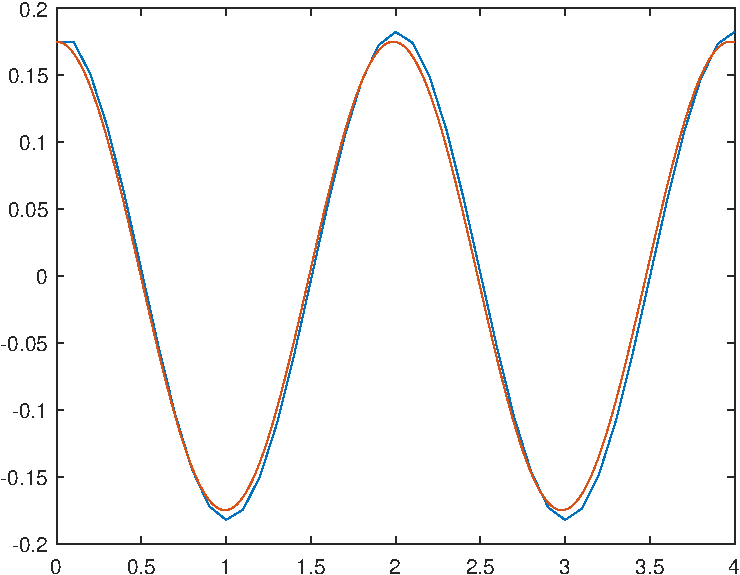
\includegraphics[width=\textwidth]{papers/fem/images/loesung_rechenbsp.pdf}
    \caption{Die mit der FEM erhaltene Lösung in Blau und die analytische Lösung in Rot.}
    \label{fem:rechenbsp:loesung}
    \end{figure}
    
Der Abbildung \ref{fem:rechenbsp:loesung} kann entnommen werden, dass die erhaltene Lösung (in Blau) nicht sehr weit von der analytischen Lösung (in Rot) abweicht.
Der zugehörige Matlab-Code kann auf GitHub \cite{fem:bib:matlab} eingesehen werden.